\section{Computer Vision Methoden zur Gesichtsanalyse}
\label{Grundlagen}
Gesichtserkennung ist eine der am weitesten fortgeschrittenen Verfahren in der maschinellen Bildverarbeitung und wird ständig weiterentwickelt. Neben dem Erkennen eines Gesichts fällt darunter auch dessen Analyse wie beispielsweise die Orientierung, Übereinstimmung oder das Erkennen von Mimik.\\
Eine Standardmethode bei der Gesichtserkennung ist die Verwendung eines Neuronalen Netzes.
\subsection{Künstliches neuronales Netz}
Ein künstliches neuronales Netz besteht aus miteinander verknüpften künstlichen Neuronen. Jedes Neuron besitzt Eingangswerte und einen Ausgabewert.\\
Um die Ausgabe zu bestimmen, werden die einzelnen Eingangswerte des Neurons individuell gewichtet, mit einer Übertragungsfunktion zusammengefasst und mittels einer Schwellenwertfunktion das Ergebnis bestimmt.\\
Um die Parameter (Gewichtung und Funktionen) des Neurons zu bestimmen, werden diese zufällig initialisiert und anschließend so trainiert, dass es zu einer gegebenen Eingabe das gewünschte Ergebnis liefert und der Fehler über dem gesamten Trainingsdatensatz minimal wird.\\
Soll ein gesamtes Netz trainiert werden, so wird jedes einzelne Neuron zufällig initialisiert und anschließend so angepasst, dass der Fehler des Netzes auf dem Trainingsdatensatz minimal wird.
\cite{Maschin_Neuron}
\subsection{Convolutional Neural Network (CNN)}
CNNs definieren in vielen Anwendungsbereichen den Stand der Technik. Sie sind eine Weiterentwicklung der neuronalen Netze und werden unter anderem bei der Bild- und Spracherkennung eingesetzt. Als Erweiterung wird eine gewichtete Faltungen der Eingabe als Eingabeparameter für das neuronale Netz verwendet.\\
Ein CNN kann in zwei Bereiche aufgeteilt werden, Feature Extraktion und Klassifizierung.\\
Bei der Feature Extraktion werden verschiedene Faltungskern und Komprimierungen auf den Eingabeinformationen angewendet um die Informationen für den zweiten Teil der Klassifizierung aufzubereiten. Durch die Faltung werden die Information aus den umliegenden Punkten eines Bereiches zusammengefasst und komprimiert an die nächste Schicht weitergegeben. Der Faltungskern kann je nach Anwendung beliebig gestaltet sein, so ist z.B. eine Glättung durch einen Gauß-Kernel oder Kantendetektion durch einen Kirsch-Operator möglich.\\
Im zweiten Teil, der Klassifizierung, werden nun alle vorhanden und zusammenführten Informationen ausgewertet, um das Ergebnis für die Eingabe zu erhalten.\\
Gelernt werden kann jeder einzelne Kernel für sich und die jeweiligen Bewertungen der Kernel und Neuronen.
\cite{pdf_CNN}\cite{wiki_CNN}
\begin{figure}
	\centering
	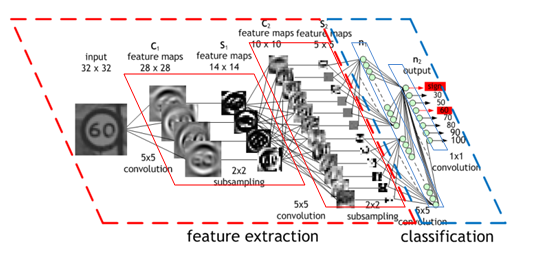
\includegraphics[width=0.9\linewidth]{img/cnn}
	\caption{Beispiel für den Aufbau eines CNN zur Klassifizierung.\\Zu sehen ist das Erkennen einer Zahl auf einem Straßenschild. Bild von \cite{bild_CNN}}
	\label{img_cnn}
\end{figure}
\subsection{Constrained Local Model (CLM)}
In Constrained Local Modellen wird die Erkennung eines Objektes in die Erkennung einzelner charakteristischer Teilpunkt, der sogenannter Landmarks, aufgespalten. Dieses Verfahren eigenen sich deshalb besonders dazu deformierbare Objekte zu erkennen.\\
Um mehrere Punkte eines Objektes zu lokalisieren wird eine Wahrscheinlichkeitskarte der einzelnen Teilpunkte relativ zueinander gelernt. Auf dem Eingabebild wird dann die Ähnlichkeit der Bildregionen mit den gesuchten Punkten quantifiziert, die die Ähnlichkeit der Darstellung angibt. Anschließend wird die optimale Kombination aus Bildähnlichkeit und der Lage aller Punkte zueinander bestimmt.\\
Diese Art der Bestimmung von positionsabhängigen Punkten ist ziemlich zuverlässig und dennoch dynamisch genug um auch mit kleinen Veränderungen zurecht zu kommen.\\
Dies ist wichtig bei der Detektion von leicht verformbaren Objekten wie beispielsweise Gesichter und ist zuverlässiger als das Active Appearance Model (AAM).
\cite{pdf_CLM}
\subsection{Constrained Local Neural Fields (CLNF)}
Bei CLNF handelt es sich um einen Gesichtsdetektor. Für die Detektion wird für jedes Merkmal ein eigener Detektor eingesetzt der auf einem Bildbereich arbeitet und eine Wahrscheinlichkeitskarte für dieses Merkmal erstellt.\\
Als nächster Schritt werden die Ergebnisse der Detektoren mit einer Karte der Position aller Landmarks, entsprechend dem Vorgehen eines CLM, verglichen.
\cite{CLNF}
\subsection{Active Appearance Model (AAM)}
Dies ist ein Verfahren der Bildverarbeitung um Übereinstimmungen zu einem Modell zu finden. Dazu wird aus dem Trainingsdatensatz eine typische \glqq durchschnittliche\grqq Form eines Objektes, sowie die Faktoren der wichtigsten möglichen Veränderungen der Form ermittelt. So können beispielsweise alle Merkmale, die ein Gesichts als männlich oder weiblich charakterisieren in einem Abweichungsvektor zusammengefasst und durch einen einzigen Gewichtungsparameter beschrieben werden.\\
Soll nun zu einem Eingabebild die Übereinstimmung ermittelt werden, so müssen nur die wichtigsten Veränderungsfaktoren angepasst werden. Dies ist ein bedeutend kleinerer Parameterraum als alle Landmarks einzeln anzupassen. Sind dennoch Unterschiede zur Eingabe vorhanden, liegen diese an der Erscheinung des Objektes.
\cite{wiki_AAM}
\newpage
\subsection{Patch Experts}
Das Patch Experts ist ein Bewertungsverfahren um die Wahrscheinlichkeit zu ermitteln, dass ein Landmark an einer bestimmten Stelle im Bild dargestellt wird. Für die Bestimmung wird ein ganzer Bereich um diese Position herum ausgewertet, um Ergebnisse auf einen Teilen eines Pixels genau zu bestimmen.
\cite{CLNF}
\subsection{Non-maximum suppression  (NMS)}
Das NMS ist ein Verfahren um ein lokales Maximum zu bestimmen und kann z.B. in einem Bild eingesetzt werden um Kanten exakter zu bestimmen.\\
Als Eingabe für das Verfahren zur exakten Bestimmung einer Kante, wird das Ergebnis eines Kantendetektor z.B. Kirsch-Operator verwendet. Dabei gibt die Höhe des Farbwertes eines Pixels an, wie nahe es an einer Kante im Originalbild liegen. Bei der Verarbeitung wird nun der Farbwert jedes einzelnen Pixels des Eingabebildes mit seinen umliegenden verglichen und sollte dieser Wert nicht maximal sein auf Null gesetzt.\\
Auf diese Weise bleibt nur noch ein Kantenpixel übrig. Wird das Verfahren auf die Bestimmung von Boxen eingesetzt, so wird jene Fläche bestimmt die von allen am ehesten beschreiben wird.
\cite{NMS}\cite{wiki_Canny}
\subsection{Point Distribution Model (PDM) \& Generalized Adaptive View-based Appearance Model (GAVAM)}
Mit einem Point Distribution Model (PDM) können verformbare Objekte modelliert werden. Dabei wird die durchschnittliche Form $\overline{X}$ des Objekts anhand der Eingabe bestimmt und eine Matrix $P$ von Eigenvektoren ermittelt, um die möglichen Deformierungen darzustellen.
\begin{align*}
X &= \overline{X}+P\cdot b
\end{align*}
Somit können durch einen Skalierungsvektor $b$ alle möglichen Eingabeformen $X$ des Objektes aus dem Durchschnittsmodell wiederhergestellt werden. Zur Vereinfachung reicht es, die signifikantesten Eigenvektoren in $P$ aufzunehmen und dennoch $X$ ausreichend genau beschreiben zu können.\\
Ist bekannt welche Art der Verformung durch den Eingenvektor dargestellt wird, z.B. eine bestimmte Orientierung, so kann anhand des Skalierungsvektors die Rotation der Eingabe bestimmt werden, siehe Generalized Adaptive View-based Appearance Model (GAVAM).\\
Eine Problematik bei dieser Art der Rotationsbestimmung entsteht, wenn die Lösung nicht eindeutig ist. Dies kann daran liegen, dass unter Umständen durch verschiedene Gewichtungskombinationen die selbe Darstellung erzielt wird oder das eine nicht erfasste Verformung des Objektes stattgefunden hat, wodurch immer eine Abweichung zu allen Kombinationen entsteht.\\
Dieses Problem der Verformung tritt bei Berechnungen von Gesichter auf, da immer eine Veränderung z.B. der Mundwinkel oder Augenlider vorhanden ist.
\cite{pdf_PDM}\cite{pdf_GAVAM}\cite{wiki_PDM}